\section{HDASSPlay\-List\-Item Class Reference}
\label{classHDASSPlayListItem}\index{HDASSPlayListItem@{HDASSPlayListItem}}
{\tt \#include $<$hdassplaylistitem.h$>$}



\subsection{Detailed Description}
\begin{Desc}
\item[Author:]sonicat \end{Desc}




Definition at line 26 of file hdassplaylistitem.h.\subsection*{Public Member Functions}
\begin{CompactItemize}
\item 
{\bf HDASSPlay\-List\-Item} (QList\-View $\ast$parent=0, const QString \&text=0, Type tt=Radio\-Button\-Controller)
\item 
{\bf $\sim$HDASSPlay\-List\-Item} ()
\item 
void {\bf setup} ()
\item 
{\bf HDASSPlay\-List\-Item} (QList\-View $\ast$parent=0, const QString \&text=0)
\item 
{\bf $\sim$HDASSPlay\-List\-Item} ()
\item 
void {\bf setup} ()
\end{CompactItemize}


\subsection{Constructor \& Destructor Documentation}
\index{HDASSPlayListItem@{HDASSPlay\-List\-Item}!HDASSPlayListItem@{HDASSPlayListItem}}
\index{HDASSPlayListItem@{HDASSPlayListItem}!HDASSPlayListItem@{HDASSPlay\-List\-Item}}
\subsubsection{\setlength{\rightskip}{0pt plus 5cm}HDASSPlay\-List\-Item::HDASSPlay\-List\-Item (QList\-View $\ast$ {\em parent} = 0, const QString \& {\em text} = 0, Type {\em tt} = Radio\-Button\-Controller)}\label{classHDASSPlayListItem_HDASSPlayListItema0}




Definition at line 22 of file hdassplaylistitem.cpp.

References setup().



\footnotesize\begin{verbatim}22                                                                                         : QCheckListItem(parent,text,tt)
23 {
24   setup();
25 }
\end{verbatim}\normalsize 


Here is the call graph for this function:\begin{figure}[H]
\begin{center}
\leavevmode
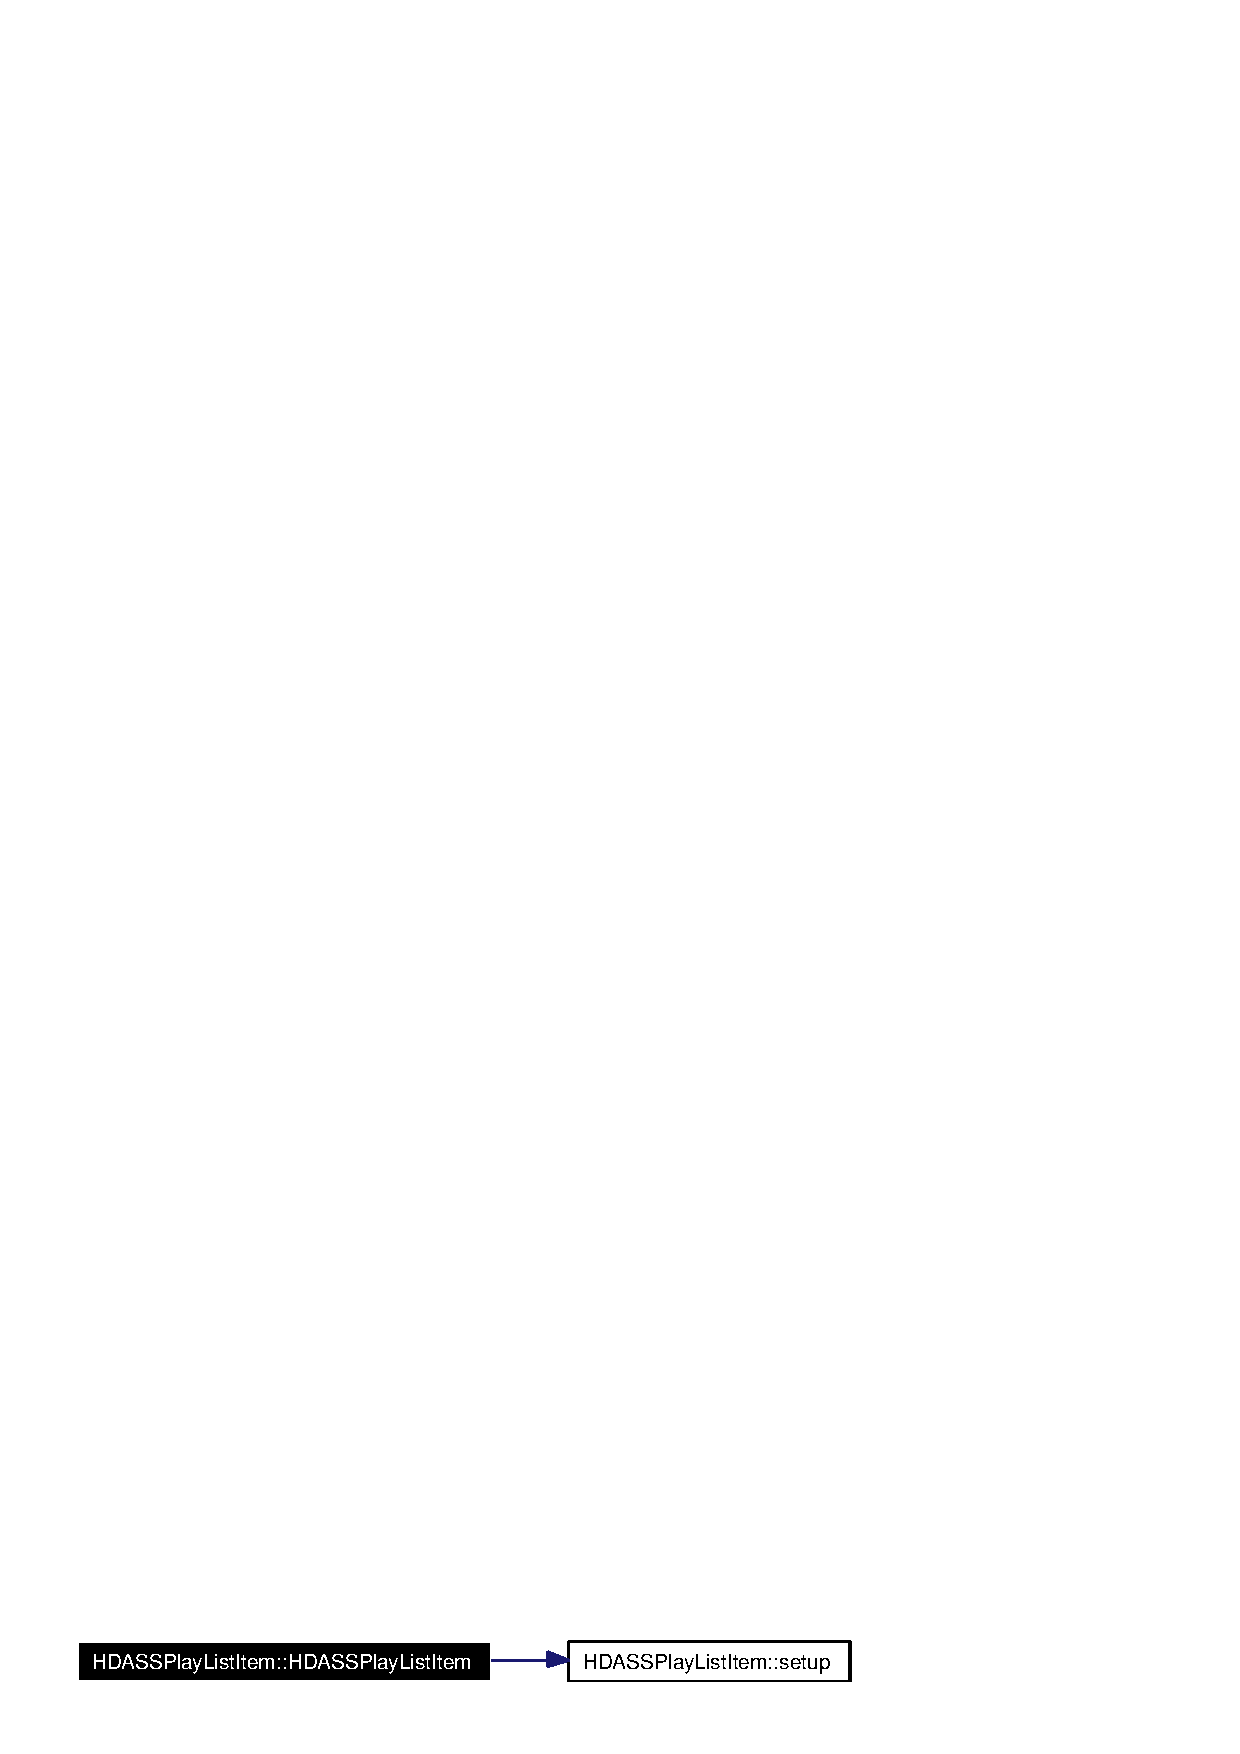
\includegraphics[width=204pt]{classHDASSPlayListItem_HDASSPlayListItema0_cgraph}
\end{center}
\end{figure}
\index{HDASSPlayListItem@{HDASSPlay\-List\-Item}!~HDASSPlayListItem@{$\sim$HDASSPlayListItem}}
\index{~HDASSPlayListItem@{$\sim$HDASSPlayListItem}!HDASSPlayListItem@{HDASSPlay\-List\-Item}}
\subsubsection{\setlength{\rightskip}{0pt plus 5cm}HDASSPlay\-List\-Item::$\sim${\bf HDASSPlay\-List\-Item} ()}\label{classHDASSPlayListItem_HDASSPlayListItema1}




Definition at line 27 of file hdassplaylistitem.cpp.



\footnotesize\begin{verbatim}28 {
29 
30 }
\end{verbatim}\normalsize 
\index{HDASSPlayListItem@{HDASSPlay\-List\-Item}!HDASSPlayListItem@{HDASSPlayListItem}}
\index{HDASSPlayListItem@{HDASSPlayListItem}!HDASSPlayListItem@{HDASSPlay\-List\-Item}}
\subsubsection{\setlength{\rightskip}{0pt plus 5cm}HDASSPlay\-List\-Item::HDASSPlay\-List\-Item (QList\-View $\ast$ {\em parent} = 0, const QString \& {\em text} = 0)}\label{classHDASSPlayListItem_HDASSPlayListItema3}




Definition at line 22 of file src/hdassplaylistitem.cpp.

References setup().



\footnotesize\begin{verbatim}22                                                                                : QListViewItem(parent,text)
23 {
24   setup();
25 }
\end{verbatim}\normalsize 


Here is the call graph for this function:\begin{figure}[H]
\begin{center}
\leavevmode
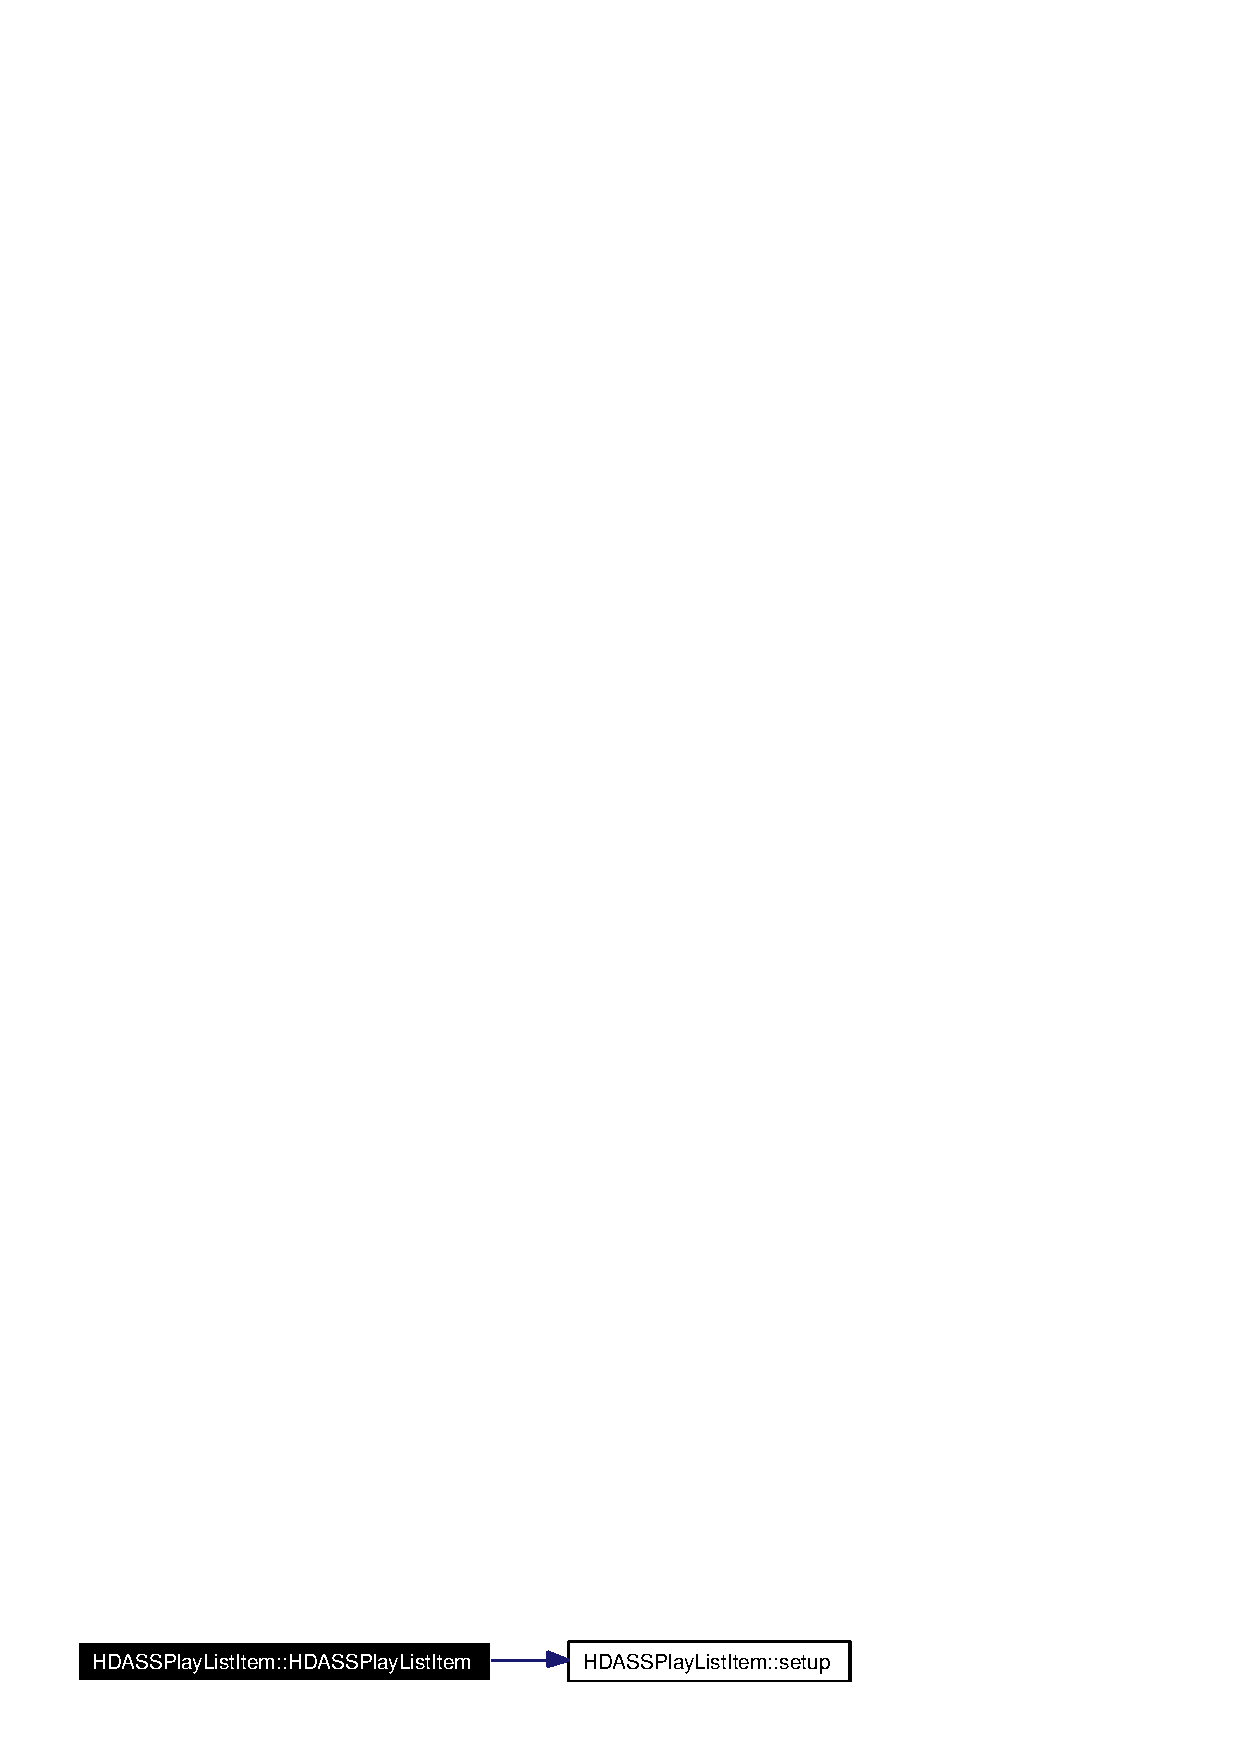
\includegraphics[width=204pt]{classHDASSPlayListItem_HDASSPlayListItema3_cgraph}
\end{center}
\end{figure}
\index{HDASSPlayListItem@{HDASSPlay\-List\-Item}!~HDASSPlayListItem@{$\sim$HDASSPlayListItem}}
\index{~HDASSPlayListItem@{$\sim$HDASSPlayListItem}!HDASSPlayListItem@{HDASSPlay\-List\-Item}}
\subsubsection{\setlength{\rightskip}{0pt plus 5cm}HDASSPlay\-List\-Item::$\sim${\bf HDASSPlay\-List\-Item} ()}\label{classHDASSPlayListItem_HDASSPlayListItema4}




\subsection{Member Function Documentation}
\index{HDASSPlayListItem@{HDASSPlay\-List\-Item}!setup@{setup}}
\index{setup@{setup}!HDASSPlayListItem@{HDASSPlay\-List\-Item}}
\subsubsection{\setlength{\rightskip}{0pt plus 5cm}void HDASSPlay\-List\-Item::setup ()}\label{classHDASSPlayListItem_HDASSPlayListItema5}


\index{HDASSPlayListItem@{HDASSPlay\-List\-Item}!setup@{setup}}
\index{setup@{setup}!HDASSPlayListItem@{HDASSPlay\-List\-Item}}
\subsubsection{\setlength{\rightskip}{0pt plus 5cm}void HDASSPlay\-List\-Item::setup ()}\label{classHDASSPlayListItem_HDASSPlayListItema2}




Definition at line 32 of file hdassplaylistitem.cpp.

Referenced by HDASSPlay\-List\-Item().



\footnotesize\begin{verbatim}33 {
34   QCheckListItem::setup();
35   setHeight(40);
36 }
\end{verbatim}\normalsize 


The documentation for this class was generated from the following files:\begin{CompactItemize}
\item 
{\bf hdassplaylistitem.h}\item 
{\bf src/hdassplaylistitem.h}\item 
{\bf hdassplaylistitem.cpp}\item 
{\bf src/hdassplaylistitem.cpp}\end{CompactItemize}
